% ============================================================
%  يُترجَم بـ XeLaTeX  (في Overleaf: Menu → Compiler → XeLaTeX)
%  الخط: Amiri (متوفر في Overleaf، أو حمّله من github.com/aliftype/amiri)
% ============================================================
\documentclass[12pt,a4paper]{article}
\usepackage[a4paper,margin=1.7cm,top=2.3cm,bottom=2.9cm,headheight=15pt,footskip=1.5cm]{geometry}
\usepackage{amsmath,amssymb}
\usepackage{icomma}
\usepackage[english,bidi=default,layout=lists]{babel}
\babelprovide[import,main]{arabic}
\babelfont{rm}[Scale=1.08]{Amiri}
\babelfont{sf}[Scale=1.08]{Amiri}
\usepackage[most]{tcolorbox}
\usepackage{tikz}
\usetikzlibrary{arrows.meta,calc,shadings}
\usepackage{array}
\usepackage{colortbl}
\usepackage{fancyhdr}
\usepackage{titlesec}
\usepackage{enumitem}
\usepackage{collcell}
\usepackage{needspace}
\usepackage{etoolbox}
\newcolumntype{C}{>{\collectcell\ar}c<{\endcollectcell}}
\pretocmd{\section}{\Needspace{15\baselineskip}}{}{}
\pretocmd{\subsection}{\Needspace{11\baselineskip}}{}{}

\definecolor{cDef}{HTML}{1F4E9C}
\definecolor{cThm}{HTML}{B3261E}
\definecolor{cRem}{HTML}{2E7D32}
\definecolor{cEx}{HTML}{C76B00}
\definecolor{cMeth}{HTML}{6A1B9A}
\definecolor{cSol}{HTML}{00695C}
\definecolor{cSec}{HTML}{1F3A68}

\titleformat{\section}{\Large\bfseries\color{cSec}}{\thesection.}{0.6em}{}[{\color{cSec!60}\titlerule[1pt]}]
\titleformat{\subsection}{\large\bfseries\color{cThm!85!black}}{\thesubsection.}{0.5em}{}
\titlespacing*{\section}{0pt}{14pt}{8pt}
\titlespacing*{\subsection}{0pt}{10pt}{5pt}
\setlength{\parindent}{0pt}
\setlength{\parskip}{4pt}
\setlist{itemsep=2pt,topsep=3pt}

\newtcolorbox{arbox}[3][]{enhanced,
  colback=#2!5,colframe=#2!80!black,arc=2mm,boxrule=0.8pt,
  left=6pt,right=6pt,top=8pt,bottom=5pt,
  fonttitle=\bfseries,coltitle=white,
  title={\foreignlanguage{arabic}{#3}},
  attach boxed title to top right={xshift=-5mm,yshift=-3mm},
  boxed title style={colback=#2!80!black,arc=1.5mm,boxrule=0pt},
  before upper={\selectlanguage{arabic}},
  before skip=8pt,after skip=8pt,breakable,#1}
\newenvironment{BOX}[2]{\begin{otherlanguage}{english}\begin{arbox}{#1}{#2}}{\end{arbox}\end{otherlanguage}}
\newenvironment{tarif}[1][تعريف]{\begin{BOX}{cDef}{#1}}{\end{BOX}}
\newenvironment{khassia}[1][خاصية]{\begin{BOX}{cThm}{#1}}{\end{BOX}}
\newenvironment{molahada}[1][ملاحظة]{\begin{BOX}{cRem}{#1}}{\end{BOX}}
\newenvironment{mithal}[1][مثال]{\begin{BOX}{cEx}{#1}}{\end{BOX}}
\newenvironment{tariqa}[1][طريقة]{\begin{BOX}{cMeth}{#1}}{\end{BOX}}

\newcounter{exo}
\newenvironment{tamrin}[1]{\stepcounter{exo}\begin{BOX}{cSec}{التمرين \theexo: #1}}{\end{BOX}}
\newenvironment{hal}{\Needspace{12\baselineskip}\begin{otherlanguage}{english}\begin{arbox}[breakable]{cSol}{حل التمرين \theexo}}{\end{arbox}\end{otherlanguage}}

\newenvironment{LTR}{\begin{otherlanguage}{english}}{\end{otherlanguage}}
\newcommand{\ar}[1]{\foreignlanguage{arabic}{#1}}

\renewcommand{\dots}{\mathinner{\ldotp\ldotp\ldotp}}
\renewcommand{\ldots}{\mathinner{\ldotp\ldotp\ldotp}}
\renewcommand{\cdots}{\mathinner{\cdotp\cdotp\cdotp}}
\newcommand{\N}{\mathbb{N}}
\newcommand{\Z}{\mathbb{Z}}
\newcommand{\D}{\mathbb{D}}
\newcommand{\Q}{\mathbb{Q}}
\newcommand{\R}{\mathbb{R}}
\newcommand{\pgcd}{\operatorname{PGCD}}
\newcommand{\ppcm}{\operatorname{PPCM}}

% \NLseg{a}{b}{[}{]} ; \NLright{a}{[} ; \NLleft{b}{]}  (interval on a number line)
\newcommand{\NLseg}[4]{\begin{LTR}\begin{tikzpicture}[baseline=-0.6ex]
 \draw[-{Stealth[length=2mm]},gray!70](0,0)--(3.4,0);
 \draw[line width=2pt,cThm!80!black](0.7,0)--(2.7,0);
 \node[cThm!80!black,font=\LARGE] at (0.7,0){$#3$};
 \node[cThm!80!black,font=\LARGE] at (2.7,0){$#4$};
 \node[below=3pt,font=\footnotesize] at (0.7,0){$#1$};
 \node[below=3pt,font=\footnotesize] at (2.7,0){$#2$};
\end{tikzpicture}\end{LTR}}
\newcommand{\NLright}[2]{\begin{LTR}\begin{tikzpicture}[baseline=-0.6ex]
 \draw[-{Stealth[length=2mm]},gray!70](0,0)--(3.4,0);
 \draw[line width=2pt,cThm!80!black](1.3,0)--(3.3,0);
 \node[cThm!80!black,font=\LARGE] at (1.3,0){$#2$};
 \node[below=3pt,font=\footnotesize] at (1.3,0){$#1$};
\end{tikzpicture}\end{LTR}}
\newcommand{\NLleft}[2]{\begin{LTR}\begin{tikzpicture}[baseline=-0.6ex]
 \draw[-{Stealth[length=2mm]},gray!70](0,0)--(3.4,0);
 \draw[line width=2pt,cThm!80!black](0.05,0)--(2.1,0);
 \node[cThm!80!black,font=\LARGE] at (2.1,0){$#2$};
 \node[below=3pt,font=\footnotesize] at (2.1,0){$#1$};
\end{tikzpicture}\end{LTR}}

% ---------- social-media icons (pure TikZ) ----------
\definecolor{cFB}{HTML}{1877F2}
\definecolor{cTG}{HTML}{229ED9}
\definecolor{cIG1}{HTML}{FEDA75}
\definecolor{cIG2}{HTML}{D62976}
\definecolor{cIG3}{HTML}{4F5BD5}
\newcommand{\fbicon}{\begin{LTR}\begin{tikzpicture}[baseline=-0.75ex,x=1em,y=1em]
 \fill[cFB] (0,0) circle (0.55);
 \node[white,inner sep=0,font=\usefont{TU}{lmss}{bx}{n}\small] at (0.04,-0.02) {f};
\end{tikzpicture}\end{LTR}}
\newcommand{\igicon}{\begin{LTR}
\begin{tikzpicture}[baseline=-0.75ex,x=1em,y=1em]
 \shade[lower left=cIG1,lower right=cIG2,upper left=cIG2,upper right=cIG3,rounded corners=0.28em] (-0.55,-0.55) rectangle (0.55,0.55);
 \draw[white,line width=0.09em,rounded corners=0.18em] (-0.36,-0.36) rectangle (0.36,0.36);
 \draw[white,line width=0.09em] (0,0) circle (0.17);
 \fill[white] (0.22,0.22) circle (0.05);
\end{tikzpicture}\end{LTR}}
\newcommand{\tgicon}{\begin{LTR}
\begin{tikzpicture}[baseline=-0.75ex,x=1em,y=1em]
 \fill[cTG] (0,0) circle (0.55);
 \fill[white] (-0.33,0.0) -- (0.32,0.27) -- (0.2,-0.3) -- (0.0,-0.15) -- (-0.08,-0.28) -- (-0.08,-0.08) -- cycle;
 \fill[cTG!70!black] (-0.08,-0.08) -- (0.25,0.2) -- (0.0,-0.15) -- (-0.08,-0.28) -- cycle;
\end{tikzpicture}\end{LTR}}
% page number: black box, white two-digit number, at the right of the social row
\newcommand{\PageBox}{\begin{LTR}\tikz[baseline=(p.base)]\node[fill=black,text=white,inner sep=2.5pt,minimum width=1.6em,minimum height=1.3em,font=\usefont{TU}{lmss}{bx}{n}\small](p){\ifnum\value{page}<10 0\fi\arabic{page}};\end{LTR}}
% visual left-to-right order: Telegram | Instagram | Facebook | page box
\newcommand{\SocialRow}{\begin{otherlanguage}{english}%
 \ar{\textbf{الأستاذ سوايسية هشام للرياضيات}}\ \tgicon\hfill
 \textbf{prof\_hicham\_math}\ \igicon\hfill
 \ar{\textbf{الأستاذ سوايسية هشام للرياضيات}}\ \fbicon\hspace{2.2em}\PageBox\end{otherlanguage}}

\pagestyle{fancy}
\fancyhf{}
\renewcommand{\headrulewidth}{0.6pt}
\renewcommand{\footrulewidth}{0.4pt}
% \SetHeader{right head: document title}{left head: level -- stream}
\newcommand{\SetHeader}[2]{%
 \fancyhead[C]{\parbox{\textwidth}{\ar{#1\hfill #2}}}%
 \fancyfoot[C]{\parbox{\textwidth}{\small\SocialRow}}}
\usepackage{tkz-tab}
\usepackage{multicol}
% variation / sign table (LTR)
\newenvironment{TAB}{\par\begin{center}\begin{LTR}\begin{tikzpicture}[scale=0.95,every node/.style={font=\small}]}{\end{tikzpicture}\end{LTR}\end{center}}
% grid + axes, clipped: \begin{GR}{xmin}{xmax}{ymin}{ymax}{unit cm}
\newenvironment{GR}[5]{\par\begin{center}\begin{LTR}\begin{tikzpicture}[x=#5cm,y=#5cm,font=\footnotesize]
 \draw[gray!25,very thin] (#1,#3) grid (#2,#4);
 \draw[-{Stealth[length=2mm]}] (#1,0)--(#2+0.3,0) node[below left]{$x$};
 \draw[-{Stealth[length=2mm]}] (0,#3)--(0,#4+0.3) node[below left]{$y$};
 \node[below left] at (0,0){$O$};
 \begin{scope}\clip (#1,#3) rectangle (#2,#4);}
{\end{scope}\end{tikzpicture}\end{LTR}\end{center}}
\newcommand{\Ticks}[2]{\foreach \t in {#1} \node[below,font=\scriptsize] at (\t,0){$\t$}; \foreach \t in {#2} \node[left,font=\scriptsize] at (0,\t){$\t$};}
\newcommand{\bx}[1]{\ensuremath{\colorbox{cDef!12}{$\displaystyle #1$}}}
\newcommand{\TwoCol}[4]{\par\begin{LTR}\noindent\begin{minipage}[t]{#1\textwidth}\selectlanguage{arabic}#2\end{minipage}\hfill\begin{minipage}[t]{#3\textwidth}\selectlanguage{arabic}#4\end{minipage}\end{LTR}\par}
\newcommand{\RL}[4]{\TwoCol{#3}{#4}{#1}{#2}}  % \RL{w1}{right content}{w2}{left content}
\newcommand{\ok}{$\textcolor{cRem}{\checkmark}$}
\newcommand{\limn}{\displaystyle\lim_{n\to+\infty}}
% sub-questions, each on its own line
\newenvironment{sq}{\begin{itemize}[leftmargin=2.4em,itemsep=3pt]}{\end{itemize}}
\newcommand{\qa}{\item[(أ)]}\newcommand{\qb}{\item[(ب)]}\newcommand{\qc}{\item[(جـ)]}\newcommand{\qd}{\item[(د)]}\newcommand{\qe}{\item[(هـ)]}
\newcommand{\pa}{\par\smallskip\textbf{(أ)} }\newcommand{\pb}{\par\smallskip\textbf{(ب)} }\newcommand{\pc}{\par\smallskip\textbf{(جـ)} }\newcommand{\pd}{\par\smallskip\textbf{(د)} }\newcommand{\pe}{\par\smallskip\textbf{(هـ)} }
\newcommand{\QQ}[1]{\par\smallskip\textbf{#1.} }
\newenvironment{tmr}{\stepcounter{exo}\begin{BOX}{cSec}{تمرين محلول \theexo}}{\end{BOX}}
\newcommand{\ABC}[3]{\\[2pt]\begin{tabular}{p{0.28\textwidth}p{0.28\textwidth}p{0.28\textwidth}}(جـ) \ #3 & (ب) \ #2 & (أ) \ #1\end{tabular}}
\pretocmd{\section}{\Needspace{24\baselineskip}}{}{}
\newtcbox{\bxtbox}{on line,colback=cDef!12,colframe=cDef!12,boxrule=0pt,arc=1pt,boxsep=0pt,left=2pt,right=2pt,top=1pt,bottom=1pt}
\newcommand{\bxt}[1]{\foreignlanguage{english}{\bxtbox{\ar{#1}}}}
\usepackage{longtable}
\setlength{\LTpre}{4pt}\setlength{\LTpost}{0pt}
\newcommand{\Phase}[1]{\textbf{#1}}
\newcommand{\Fld}[2]{\textbf{#1:}\ #2}
% رأس المذكرة على نمط النموذج: إطار بعنوان «مذكرة رقم»، معلومات الحصة، ثم إطار الكفاءات
\newcommand{\ModhHead}[9]{%
\begin{LTR}
\begin{tcolorbox}[enhanced,colback=white,colframe=cThm!85!black,arc=4mm,boxrule=1pt,top=14pt,bottom=6pt,left=8pt,right=8pt,
 overlay={\node[fill=cThm!85!black,text=white,rounded corners=3mm,inner xsep=14pt,inner ysep=4pt,font=\large\bfseries] at ([yshift=0pt]frame.north){\ar{مذكرة رقم #1}};},
 before upper={\selectlanguage{arabic}}]
\begin{tabular}{@{}p{0.4\linewidth}p{0.55\linewidth}@{}}
\Fld{المستوى}{#2} & \Fld{الثانوية}{\dotfill}\\[3pt]
\Fld{المادة}{رياضيات} & \Fld{ميدان التعلم}{#3}\\[3pt]
\Fld{المدة}{#5} & \Fld{الوحدة التعلمية}{#4}\\[3pt]
\Fld{الأستاذ}{\dotfill} & \Fld{المحتوى المعرفي}{#6}\\
\end{tabular}
\end{tcolorbox}
\begin{tcolorbox}[enhanced,colback=white,colframe=cThm!85!black,arc=3mm,boxrule=0.8pt,sidebyside,sidebyside align=top,lefthand ratio=0.5,
 segmentation style={dashed,cThm!60},before upper={\selectlanguage{arabic}},before lower={\selectlanguage{arabic}}]
\textbf{الكفاءات المستهدفة:}\par #8
\tcblower
\textbf{الكفاءات القبلية:}\par #7
\end{tcolorbox}
\end{LTR}
\par\smallskip\textbf{الوسائل:} #9\par\smallskip}
\newenvironment{Sayr}{%
\begin{LTR}\renewcommand{\arraystretch}{1.25}
\begin{longtable}{|p{0.17\textwidth}|>{\centering\arraybackslash}p{0.06\textwidth}|p{0.53\textwidth}|>{\centering\arraybackslash}p{0.12\textwidth}|}
\hline\rowcolor{cThm!12}\ar{\textbf{توجيهات وتعاليق}} & \ar{\textbf{المدة}} & \ar{\textbf{سير الحصة}} & \ar{\textbf{مراحل الحصة}}\\\hline\endhead
\hline\endfoot}{\end{longtable}\end{LTR}}
% سطر في الجدول: \Row{مرحلة}{سير}{مدة}{توجيهات}
\newcommand{\Row}[4]{\ar{\small #4} & \ar{#3} & \ar{#2} & \cellcolor{cThm!8}\ar{\Phase{#1}}\\\hline}

\newcommand{\Lab}[2]{\foreignlanguage{english}{\tcbox[on line,colback=#1,colframe=#1,boxrule=0pt,arc=2pt,boxsep=1pt,left=5pt,right=5pt,top=1pt,bottom=1pt]{\ar{\textcolor{white}{\textbf{#2}}}}}}
\newcommand{\Num}[1]{\foreignlanguage{english}{\tikz[baseline=(c.base)]\node[fill=cDef,text=white,inner sep=2pt,font=\footnotesize\bfseries](c){#1};}}
\newcommand{\ck}{\ensuremath{{\color{cRem}\checkmark}}}
\newenvironment{Kad}[1]{\par\smallskip\Lab{#1}}{\par}
\SetHeader{\small\bfseries\color{cSec}مذكرات محور: الدوال المرجعية}{\small\color{cSec}السنة الأولى ثانوي -- جذع مشترك علوم وتكنولوجيا}
\begin{document}
\begin{LTR}
\begin{tcolorbox}[enhanced,colback=cThm!85!black,colframe=cThm!85!black,arc=3mm,halign=center,boxrule=0pt,top=12pt,bottom=12pt,before upper={\selectlanguage{arabic}}]
{\color{white}\fontsize{26}{32}\selectfont\bfseries مذكرات محور: الدوال المرجعية}\\[8pt]
{\color{white}\large السنة الأولى ثانوي -- جذع مشترك علوم وتكنولوجيا}\\[4pt]
{\color{white}\large 6 مذكرات (12 ساعة) -- السنة الدراسية 2026-2027}
\end{tcolorbox}
\end{LTR}
\begin{BOX}{cThm}{يتضمن هذا العمل}
\begin{enumerate}[label=\textbf{مذكرة \arabic{enumi}:},leftmargin=6em,start=23]
\item الدالة التآلفية ونسبة التزايد.
\item الدالة مربع والتمثيل بالاعتماد على دالة مرجعية.
\item الدالة مقلوب.
\item الدالة الجذر التربيعي والدالة القيمة المطلقة.
\item الدائرة المثلثية والراديان.
\item جيب وجيب تمام عدد حقيقي ، الدالتان $\sin$ و $\cos$.
\end{enumerate}
مراجع النشاطات: الكتاب المدرسي للسنة الأولى ثانوي جذع مشترك علوم وتكنولوجيا (باب الدوال المرجعية ص 82--83).
\end{BOX}
\newpage
\ModhHead{23}{1 ج م ع ت}{تحليل}{الدوال المرجعية}{02 سا}{الدالة التآلفية ونسبة التزايد}%
{\begin{itemize}\item معادلة مستقيم ومعامل التوجيه.\item اتجاه تغير دالة.\end{itemize}}%
{\begin{itemize}\item حساب نسبة تزايد دالة واستعمالها لدراسة اتجاه التغير.\item تمثيل دالة تآلفية.\end{itemize}}%
{المنهاج ، الكتاب المدرسي ، مراجع ، الحاسبة البيانية.}
\begin{Sayr}
\Row{مرحلة الانطلاق}{%
\textbf{التهيئة النفسية:} تعريفة سيارة أجرة: $100$ DA للركوب و $40$ DA لكل كيلومتر. ما ثمن رحلة طولها $x$ km؟}{10 د}{وضعية من الحياة اليومية.}
\Row{التشخيص والاكتشاف}{%
\Lab{cEx}{وضعية مقترحة}\par\ck\ $p(x)=40x+100$: دالة \textbf{تآلفية}.\par
\ck\ من أجل $a\ne b$: $\dfrac{p(b)-p(a)}{b-a}=\dfrac{40(b-a)}{b-a}=40$: الزيادة في الثمن متناسبة مع الزيادة في المسافة.\par
\ck\ $40>0$: كلما زادت المسافة زاد الثمن.\par
}{35 د}{عمل ثنائي.}
\Row{بناء المعارف}{%
\Lab{cDef}{نسبة التزايد}\ لدالة $f$ بين عددين $a\ne b$ من $D_f$: \ $\dfrac{f(b)-f(a)}{b-a}$.\par\Lab{cThm}{خاصية}\ إذا كانت نسبة التزايد موجبة تماماً على مجال $I$ فإن $f$ متزايدة تماماً على $I$ ، وإذا كانت سالبة تماماً فهي متناقصة تماماً.\par}{50 د}{نربط نسبة التزايد بمعامل التوجيه.}
\Row{}{%
\Lab{cDef}{الدالة التآلفية}\ $f(x)=ax+b$ ؛ نسبة تزايدها $a$ ، وتمثيلها مستقيم معامل توجيهه $a$.\par\Lab{cEx}{مثال}\ $f(x)=-2x+3$: نسبة التزايد $-2<0$ ، إذن $f$ متناقصة تماماً على $\R$.\par}{}{}
\Row{}{%
\Lab{cThm!80!black}{حذار}\ الدالة الخطية $x\mapsto ax$ حالة خاصة ($b=0$) ومنحناها يشمل المبدأ.}{}{}
\Row{التقويم}{%
\Lab{cEx}{تطبيق}\par\Num{1} ادرس اتجاه تغير $g(x)=\dfrac12x-4$. \Num{2} عيّن الدالة التآلفية $h$ حيث $h(1)=5$ و $h(3)=1$.\par\textbf{الحل:} \Num{1} متزايدة تماماً ($\frac12>0$) ؛ \Num{2} $a=\dfrac{1-5}{3-1}=-2$ ، $h(x)=-2x+7$.\par\textbf{واجب منزلي:} تمارين من الكتاب المدرسي.\par\smallskip\textbf{ملاحظات حول سير الحصة:} \dotfill}{25 د}{تقويم فردي.}
\end{Sayr}
\newpage
\ModhHead{24}{1 ج م ع ت}{تحليل}{الدوال المرجعية}{02 سا}{الدالة مربع والتمثيل بالاعتماد على دالة مرجعية}%
{\begin{itemize}\item نسبة التزايد.\item المتطابقات الشهيرة.\end{itemize}}%
{\begin{itemize}\item دراسة اتجاه تغير الدالة مربع وتمثيلها.\item استعمال الدالة مربع لمقارنة أعداد.\item تمثيل دالة بالاعتماد على الدالة مربع.\end{itemize}}%
{المنهاج ، الكتاب المدرسي ، مراجع ، الحاسبة البيانية.}
\begin{Sayr}
\Row{مرحلة الانطلاق}{%
\textbf{التهيئة النفسية:} مساحة مربع طول ضلعه $x$: هل تتضاعف المساحة عندما يتضاعف الطول؟}{10 د}{سؤال يثير خطأ شائعاً.}
\Row{التشخيص والاكتشاف}{%
\Lab{cEx}{مناقشة نشاط 01 صفحة 82}\par\ck\ مساحة قطعة أرض مربعة طول ضلعها $x$: $f(x)=x^2$ ، والمساحة لا تتجاوز $3600$ m² ، إذن $x\in[0;60]$.\par
\ck\ الجدول: $f(0)=0$ ، $f(10)=100$ ، $f(20)=400$ ، $f(30)=900$ ، $f(40)=1600$ ، $f(50)=2500$.\par
\ck\ كلما زاد الطول زادت المساحة ، وكلما نقص نقصت: $f$ \textbf{متزايدة} على $[0;60]$.\par
}{35 د}{جدول القيم بالحاسبة.}
\Row{بناء المعارف}{%
\Lab{cThm}{خاصية}\ الدالة مربع $x\mapsto x^2$ معرفة على $\R$ ، و $\dfrac{f(b)-f(a)}{b-a}=a+b$.\par\ck\ على $[0;+\infty[$: $a+b>0$: متزايدة تماماً ؛ على $]-\infty;0]$: $a+b<0$: متناقصة تماماً.\par
\ck\ الدالة زوجية ، ومنحناها \textbf{قطع مكافئ} رأسه المبدأ ومحور تناظره محور التراتيب.\par
\Lab{cMeth}{المقارنة}\ $-3<-2{,}5\leqslant0$ والدالة متناقصة على $]-\infty;0]$ ، إذن $(-3)^2>(-2{,}5)^2$.\par}{50 د}{نرسم المنحنى بدقة على ورق مليمتري.}
\Row{}{%
\Lab{cEx}{التمثيل بدالة مرجعية}\ منحنى $g(x)=(x-1)^2+2$ هو صورة منحنى $x^2$ بالانسحاب الذي شعاعه $\vec v(1;2)$ ، وقيمته الحدية الصغرى $2$ عند $x=1$.\par\smallskip\begin{LTR}\centering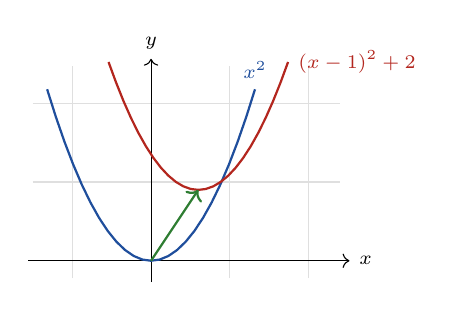
\begin{tikzpicture}[x=0.6cm,y=0.45cm,font=\scriptsize]
\draw[gray!25] (-2.5,-0.5) grid (4,5.5);
\draw[->] (-2.6,0)--(4.2,0) node[right]{$x$}; \draw[->] (0,-0.6)--(0,5.7) node[above]{$y$};
\draw[cDef,thick,domain=-2.2:2.2] plot (\x,{\x*\x}) node[above]{$x^2$};
\draw[cThm,thick,domain=-0.9:2.9] plot (\x,{(\x-1)*(\x-1)+2}) node[right]{$(x-1)^2+2$};
\draw[cRem,->,thick] (0,0)--(1,2);
\end{tikzpicture}\end{LTR}\par\Lab{cThm!80!black}{حذار}\ $x^2\geqslant x$ ليست صحيحة دائماً (مثلاً $x=0{,}5$).}{}{}
\Row{التقويم}{%
\Lab{cEx}{تطبيق}\par\Num{1} قارن $(1{,}3)^2$ و $(1{,}31)^2$ ؛ $(-0{,}7)^2$ و $(-0{,}8)^2$. \Num{2} إذا كان $-2\leqslant x\leqslant1$ فما حصر $x^2$ ؟\par\textbf{الحل:} \Num{1} $(1{,}3)^2<(1{,}31)^2$ ؛ $(-0{,}7)^2<(-0{,}8)^2$ ؛ \Num{2} $0\leqslant x^2\leqslant4$ (لأن المجال يشمل $0$).\par\textbf{واجب منزلي:} تمارين من الكتاب المدرسي.\par\smallskip\textbf{ملاحظات حول سير الحصة:} \dotfill}{25 د}{نشدد على حالة مجال يشمل $0$.}
\end{Sayr}
\newpage
\ModhHead{25}{1 ج م ع ت}{تحليل}{الدوال المرجعية}{02 سا}{الدالة مقلوب}%
{\begin{itemize}\item نسبة التزايد.\item الدالة مربع.\end{itemize}}%
{\begin{itemize}\item دراسة اتجاه تغير الدالة مقلوب وتمثيلها.\item استعمالها لمقارنة أعداد وحل متراجحات بيانياً.\end{itemize}}%
{المنهاج ، الكتاب المدرسي ، مراجع ، الحاسبة البيانية.}
\begin{Sayr}
\Row{مرحلة الانطلاق}{%
\textbf{التهيئة النفسية:} مستطيل مساحته $1$ m² وطوله $x$: ما عرضه؟ ماذا يحدث للعرض عندما يكبر الطول؟}{10 د}{وضعية هندسية.}
\Row{التشخيص والاكتشاف}{%
\Lab{cEx}{وضعية مقترحة}\par\ck\ العرض $\dfrac1x$ حيث $x>0$.\par
\ck\ الجدول: $x=0{,}5$: $2$ ؛ $x=1$: $1$ ؛ $x=2$: $0{,}5$ ؛ $x=4$: $0{,}25$: كلما كبر الطول صغر العرض.\par
}{35 د}{جدول قيم بالحاسبة.}
\Row{بناء المعارف}{%
\Lab{cThm}{خاصية}\ الدالة مقلوب $x\mapsto\dfrac1x$ معرفة على $\R^*$ ، و $\dfrac{f(b)-f(a)}{b-a}=-\dfrac1{ab}$.\par\ck\ على $]0;+\infty[$ ($ab>0$): متناقصة تماماً ؛ وعلى $]-\infty;0[$ أيضاً متناقصة تماماً.\par
\ck\ الدالة فردية ، ومنحناها \textbf{قطع زائد} مركز تناظره المبدأ.\par
\Lab{cThm!80!black}{حذار}\ الدالة مقلوب ليست متناقصة على $\R^*$ كله: $-1<1$ و $\dfrac1{-1}<\dfrac11$.\par}{50 د}{نؤكد على القيمة الممنوعة $0$.}
\Row{}{%
\Lab{cEx}{مثال}\par\ck\ $0<0{,}3<0{,}31$ ، إذن $\dfrac1{0{,}3}>\dfrac1{0{,}31}$.\par
\ck\ بيانياً: $\dfrac1x<2\iff x<0$ أو $x>\dfrac12$.\par
}{}{}
\Row{التقويم}{%
\Lab{cEx}{تطبيق}\par\Num{1} قارن $\dfrac1{-2}$ و $\dfrac1{-3}$. \Num{2} إذا كان $2\leqslant x\leqslant5$ فما حصر $\dfrac1x$ ؟\par\textbf{الحل:} \Num{1} $-3<-2<0$ والدالة متناقصة على $]-\infty;0[$: $\dfrac1{-3}>\dfrac1{-2}$ ؛ \Num{2} $\dfrac15\leqslant\dfrac1x\leqslant\dfrac12$.\par\textbf{واجب منزلي:} تمارين من الكتاب المدرسي.\par\smallskip\textbf{ملاحظات حول سير الحصة:} \dotfill}{25 د}{تقويم فردي.}
\end{Sayr}
\newpage
\ModhHead{26}{1 ج م ع ت}{تحليل}{الدوال المرجعية}{02 سا}{الدالة الجذر التربيعي والدالة القيمة المطلقة}%
{\begin{itemize}\item نسبة التزايد.\item القيمة المطلقة.\end{itemize}}%
{\begin{itemize}\item دراسة اتجاه تغير الدالة الجذر التربيعي والدالة القيمة المطلقة وتمثيلهما.\item مقارنة أعداد باستعمالهما.\end{itemize}}%
{المنهاج ، الكتاب المدرسي ، مراجع ، الحاسبة البيانية.}
\begin{Sayr}
\Row{مرحلة الانطلاق}{%
\textbf{التهيئة النفسية:} مربع مساحته $S$: ما طول ضلعه؟ ارسم بعض النقط $(S;\sqrt S)$.}{10 د}{سؤال هندسي.}
\Row{التشخيص والاكتشاف}{%
\Lab{cEx}{وضعية مقترحة}\par\ck\ طول الضلع $\sqrt S$ حيث $S\geqslant0$: $\sqrt0=0$ ، $\sqrt1=1$ ، $\sqrt4=2$ ، $\sqrt9=3$.\par
\ck\ كلما كبرت المساحة كبر الضلع ، لكن بشكل أبطأ.\par
}{35 د}{جدول قيم.}
\Row{بناء المعارف}{%
\Lab{cThm}{الجذر التربيعي}\ $x\mapsto\sqrt x$ معرفة على $[0;+\infty[$ ، و $\dfrac{f(b)-f(a)}{b-a}=\dfrac1{\sqrt a+\sqrt b}>0$: متزايدة تماماً على $[0;+\infty[$. منحناها نصف قطع مكافئ.\par\Lab{cThm}{القيمة المطلقة}\ $x\mapsto|x|$ معرفة على $\R$: $|x|=-x$ على $]-\infty;0]$ (متناقصة) و $|x|=x$ على $[0;+\infty[$ (متزايدة). زوجية ، ومنحناها نصفا مستقيمين.\par}{50 د}{نرسم المنحنيات الثلاثة $x^2$ ، $x$ ، $\sqrt x$ في نفس المعلم.}
\Row{}{%
\Lab{cEx}{مثال}\par\ck\ $2{,}5<2{,}6$ ، إذن $\sqrt{2{,}5}<\sqrt{2{,}6}$.\par
\ck\ من أجل $0\leqslant x\leqslant1$: $x^2\leqslant x\leqslant\sqrt x$ (نقارن المنحنيات الثلاثة).\par
\Lab{cThm!80!black}{حذار}\ $\sqrt{x^2}=|x|$ وليس $x$.}{}{}
\Row{التقويم}{%
\Lab{cEx}{تطبيق}\par\Num{1} إذا كان $1\leqslant x\leqslant9$ فما حصر $\sqrt x$ ؟ \Num{2} ارسم منحنى $g(x)=|x-2|$ انطلاقاً من منحنى $|x|$.\par\textbf{الحل:} \Num{1} $1\leqslant\sqrt x\leqslant3$ ؛ \Num{2} انسحاب شعاعه $2\vec i$.\par\textbf{واجب منزلي:} تمارين من الكتاب المدرسي.\par\smallskip\textbf{ملاحظات حول سير الحصة:} \dotfill}{25 د}{تقويم فردي.}
\end{Sayr}
\newpage
\ModhHead{27}{1 ج م ع ت}{تحليل}{الدوال المرجعية}{02 سا}{الدائرة المثلثية والراديان}%
{\begin{itemize}\item جيب وجيب تمام زاوية حادة في مثلث قائم.\item محيط الدائرة.\end{itemize}}%
{\begin{itemize}\item معرفة الدائرة المثلثية.\item التحويل من الدرجة إلى الراديان وبالعكس.\item تعليم نقطة على الدائرة المثلثية.\end{itemize}}%
{المنهاج ، الكتاب المدرسي ، مراجع ، أدوات الهندسة.}
\begin{Sayr}
\Row{مرحلة الانطلاق}{%
\textbf{التهيئة النفسية:} التذكير بـ $\cos30^\circ$ ، $\sin30^\circ$ ، $\cos45^\circ$ في مثلث قائم.}{10 د}{تذكير بالمتوسط.}
\Row{التشخيص والاكتشاف}{%
\Lab{cEx}{مناقشة النشاطين 02 و 03 صفحة 82 ، ونشاط 04 صفحة 83}\par\ck\ في ربع دائرة نصف قطرها $1$: النقطة $M$ إحداثياها $(\cos\alpha;\sin\alpha)$.\par
\ck\ الدائرة المثلثية: مركزها $O$ ، نصف قطرها $1$ ، موجهة في الاتجاه المباشر (عكس عقارب الساعة).\par
\ck\ طول القوس $\overset{\frown}{IJ}$ هو ربع المحيط: $\dfrac{2\pi}{4}=\dfrac\pi2$.\par
}{35 د}{عمل بالمدور والمنقلة.}
\Row{بناء المعارف}{%
\Lab{cDef}{الراديان}\ قيس الزاوية المركزية التي تحصر قوساً طوله يساوي نصف القطر. \ \bx{180^\circ=\pi\ \text{rad}}.\par\Lab{cEx}{مثال}\ $30^\circ=\dfrac\pi6$ ؛ $45^\circ=\dfrac\pi4$ ؛ $60^\circ=\dfrac\pi3$ ؛ $90^\circ=\dfrac\pi2$ ؛ $120^\circ=\dfrac{2\pi}3$.\par}{50 د}{نرسم الدائرة المثلثية بدقة.}
\Row{}{%
\Lab{cThm}{خاصية}\ على الدائرة المثلثية طول القوس يساوي قيس الزاوية بالراديان.\par\Lab{cRem}{ملاحظات}\ ندوّر في الاتجاه المباشر للأعداد الموجبة وفي الاتجاه غير المباشر للسالبة.\par\smallskip\begin{LTR}\centering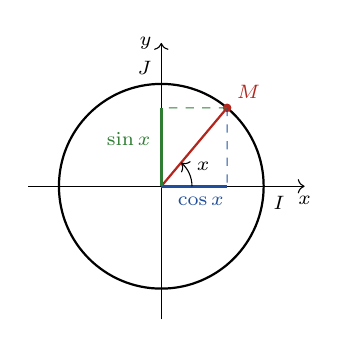
\begin{tikzpicture}[scale=1.3,font=\scriptsize]
\draw[->] (-1.3,0)--(1.4,0) node[below]{$x$}; \draw[->] (0,-1.3)--(0,1.4) node[left]{$y$};
\draw[thick] (0,0) circle (1);
\draw[cThm,thick] (0,0)--(50:1); \fill[cThm] (50:1) circle (1.2pt) node[above right]{$M$};
\draw[cDef,dashed] (50:1)--(0.643,0); \draw[cRem,dashed] (50:1)--(0,0.766);
\draw[cDef,very thick] (0,0)--(0.643,0) node[below,pos=0.6]{$\cos x$};
\draw[cRem,very thick] (0,0)--(0,0.766) node[left,pos=0.6]{$\sin x$};
\draw[->] (0.3,0) arc (0:50:0.3); \node at (25:0.45){$x$};
\node[below right] at (1,0){$I$}; \node[above left] at (0,1){$J$};
\end{tikzpicture}\end{LTR}\par}{}{}
\Row{}{%
\Lab{cThm!80!black}{حذار}\ لا نخلط بين الدرجة والراديان في الحاسبة (وضع DEG أو RAD).}{}{}
\Row{التقويم}{%
\Lab{cEx}{تطبيق}\par\Num{1} حوّل $150^\circ$ و $\dfrac{5\pi}{4}$. \Num{2} علّم على الدائرة المثلثية النقط المرفقة بـ $\dfrac\pi2$ ، $\pi$ ، $-\dfrac\pi2$.\par\textbf{الحل:} \Num{1} $150^\circ=\dfrac{5\pi}6$ ؛ $\dfrac{5\pi}{4}=225^\circ$ ؛ \Num{2} $J$ ، $I_1(-1;0)$ ، $J_1(0;-1)$.\par\textbf{واجب منزلي:} تمارين من الكتاب المدرسي.\par\smallskip\textbf{ملاحظات حول سير الحصة:} \dotfill}{25 د}{تقويم فردي.}
\end{Sayr}
\newpage
\ModhHead{28}{1 ج م ع ت}{تحليل}{الدوال المرجعية}{02 سا}{جيب وجيب تمام عدد حقيقي ، الدالتان $\sin$ و $\cos$}%
{\begin{itemize}\item الدائرة المثلثية والراديان.\end{itemize}}%
{\begin{itemize}\item تعريف $\cos x$ و $\sin x$ و $\tan x$ لعدد حقيقي $x$.\item معرفة اتجاه تغير الدالتين جيب وجيب تمام وتمثيلهما.\end{itemize}}%
{المنهاج ، الكتاب المدرسي ، مراجع ، الحاسبة البيانية.}
\begin{Sayr}
\Row{مرحلة الانطلاق}{%
\textbf{التهيئة النفسية:} ما النقطة المرفقة بالعدد $2\pi$ ؟ و $\dfrac\pi6+2\pi$ ؟}{10 د}{سؤال يقود إلى الدورية.}
\Row{التشخيص والاكتشاف}{%
\Lab{cEx}{مناقشة نشاط 05 صفحة 83}\par\ck\ بلف المستقيم العددي حول الدائرة المثلثية نرفق بكل عدد حقيقي $x$ نقطة وحيدة $M$.\par
\ck\ الأعداد $x$ و $x+2\pi$ و $x-2\pi$ $\ldots$ لها نفس النقطة.\par
\ck\ $\dfrac{7\pi}3=\dfrac\pi3+2\pi$ و $-\dfrac{13\pi}6=\dfrac{11\pi}{6}-4\pi$.\par
}{35 د}{نستعمل الدائرة المثلثية المرسومة على السبورة.}
\Row{بناء المعارف}{%
\Lab{cDef}{تعريف}\ إذا كانت $M$ النقطة المرفقة بـ $x$ فإن $\cos x$ فاصلتها و $\sin x$ ترتيبها ، و $\tan x=\dfrac{\sin x}{\cos x}$ ($\cos x\ne0$).\par\Lab{cThm}{خاصية}\ $-1\leqslant\cos x\leqslant1$ ؛ $-1\leqslant\sin x\leqslant1$ ؛ \bx{\cos^2x+\sin^2x=1} ؛ $\cos(x+2\pi)=\cos x$ ؛ $\sin(x+2\pi)=\sin x$ ؛ $\cos(-x)=\cos x$ ؛ $\sin(-x)=-\sin x$.\par}{50 د}{نرسم المنحنيين بالحاسبة البيانية.}
\Row{}{%
\Lab{cThm}{اتجاه التغير}\ $\cos$ متناقصة على $[0;\pi]$ ؛ $\sin$ متزايدة على $\Big[-\dfrac\pi2;\dfrac\pi2\Big]$ ؛ نكمل المنحنيين بالدورية.\par\Lab{cEx}{مثال}\ $\cos\dfrac\pi3=\dfrac12$ ، $\sin\dfrac\pi3=\dfrac{\sqrt3}2$ ؛ $\cos\dfrac{7\pi}{3}=\cos\dfrac\pi3=\dfrac12$.\par}{}{}
\Row{}{%
\Lab{cThm!80!black}{حذار}\ $\cos^2x$ تعني $(\cos x)^2$ وليس $\cos(x^2)$.}{}{}
\Row{التقويم}{%
\Lab{cEx}{تطبيق}\par عيّن: $\cos(-2\pi)$ ، $\sin\Big(-\dfrac\pi2\Big)$ ، $\cos\dfrac{3\pi}2$ ، $\sin\dfrac{3\pi}2$ ، $\cos0$ ، $\sin0$.\par\textbf{الحل:} $1$ ؛ $-1$ ؛ $0$ ؛ $-1$ ؛ $1$ ؛ $0$.\par\textbf{واجب منزلي:} تمارين حوصلة المحور من الكتاب المدرسي.\par\smallskip\textbf{ملاحظات حول سير الحصة:} \dotfill}{25 د}{نهاية المحور: فرض أو تمارين حوصلة.}
\end{Sayr}
\end{document}
